\chapter{Sviluppare Kargo}
\label{chap:progettazione-codifica}

\textit{Il presente capitolo documenta le fasi operative del progetto Kargo, illustrando il metodo di lavoro adottato e il percorso di sviluppo che ha condotto alla realizzazione dell'applicativo. Attraverso l'analisi del ciclo di vita del software e delle principali sfide progettuali, descrivo il percorso che ha condotto dalla definizione dei requisiti iniziali alla realizzazione e validazione dell'applicativo.}

\section{Metodologia di lavoro e interazione}
\label{sec:metodologia_lavoro}

Per garantire il corretto avanzamento del progetto all'interno del limitato orizzonte temporale dello \textit{stage}, ho definito con il tutor aziendale un perimetro metodologico chiaro, stabilendo le regole di comunicazione e i criteri di validazione fin dal primo giorno di attività.

\subsection{Modello di interazione aziendale e versionamento}
\label{subsec:interazione_aziendale}

Operando come unica risorsa di sviluppo dedicata al progetto Kargo, ho instaurato con il tutor --- che ricopriva il ruolo di \textit{stakeholder} di riferimento --- una comunicazione fluida e continua, agevolata dalla vicinanza fisica dei nostri uffici. Abbiamo optato per un approccio interattivo privo di scadenze formali rigide, prediligendo allineamenti mirati al bisogno.

Di fronte a ostacoli tecnici o dubbi implementativi, evitavo di presentare semplicemente l'anomalia, ma sottoponevo al tutor una procedura strutturata in tre fasi:
\begin{enumerate}
    \item Dimostrazione della comprensione della problematica.
    \item Formulazione di una o più ipotesi di risoluzione, giustificate dallo studio teorico delle tecnologie coinvolte.
    \item Applicazione concreta della soluzione all'interno del codice per dimostrarne il funzionamento.
\end{enumerate}

A seguito di questa dimostrazione, il tutor mi forniva i propri riscontri. Le direttive ricevute differivano sensibilmente tra \textit{frontend} e \textit{backend}: il livello di presentazione subiva controlli estetici e funzionali stringenti per soddisfare i requisiti visivi del committente finale, mentre sul livello logico ho beneficiato di ampia libertà organizzativa e decisionale.

Sul piano del tracciamento del codice sorgente, l'azienda mi ha richiesto di mantenere l'approccio di storicizzazione manuale descritto nella Sezione~\ref{subsec:transizione_architetturale}. Nonostante la mia familiarità con i moderni sistemi di versionamento come Git, la mancanza di procedure interne già consolidate per queste piattaforme ha indotto il tutor a optare per il salvataggio basato su copie di \textit{backup}. Ho quindi separato fisicamente il progetto in tre \textit{directory} autonome: una cartella per il \textit{backend} sviluppato in ambiente Visual Studio con .NET Web API, una per il \textit{frontend} inizializzato con Vite per l'ecosistema React, e una terza dedicata alla documentazione tecnica. Sebbene avessi evidenziato alcune criticità in termini di manutenibilità, questo vincolo ha comportato in alcune occasioni un impiego di tempo operativo aggiuntivo per la ristrutturazione e il riordino dei \textit{file}, rallentando il flusso di sviluppo produttivo.

\subsection{Metodologia di sviluppo personale e tracciamento}
\label{subsec:sviluppo_personale}

In assenza di piattaforme digitali per la gestione dei compiti --- quali \textit{board} Kanban o \textit{software} di \textit{ticketing} --- e in assenza di una struttura di \gls{project-management}, ovvero la disciplina che organizza metodologicamente l'avvio, la pianificazione e l'esecuzione di progetti aziendali, ho ideato un sistema organizzativo personale basato su supporto cartaceo per governare i cicli di sviluppo quotidiani.

Ho scelto il supporto analogico per la sua capacità di minimizzare il carico cognitivo associato all'uso di \textit{software} di gestione esterna, permettendomi di mantenere elevata la concentrazione sulla logica applicativa. Questa metodologia mi ha consentito di riflettere sulle regole di dominio prima della loro implementazione: la stesura a mano mi ha obbligato a sintetizzare le regole di \textit{business} prima di tradurle nel codice, garantendo che ogni riga implementata fosse funzionale a un obiettivo di dominio chiaro.

Per compensare la mancanza di scadenze aziendali formali e soddisfare i requisiti di tracciabilità metodologica, ogni giornata lavorativa iniziava con la stesura di un elenco di obiettivi, separando rigidamente le mansioni obbligatorie, necessarie per il proseguimento del flusso primario, da quelle opzionali. Per implementare ogni singola funzionalità, ho impiegato specifici strumenti di analisi e verifica, quali diagrammi \gls{uml} per la modellazione e interfacce di \textit{test} HTTP per il collaudo. Per considerare un incarico effettivamente concluso, ho definito tre criteri di completamento, che ho monitorato costantemente per ogni singola attività:
\begin{itemize}
    \item \textbf{Completamento funzionale:} l'applicativo doveva superare con successo l'operazione richiesta dal requisito.
    \item \textbf{Documentazione contestuale:} il codice sorgente doveva presentare commenti esplicativi in ogni nodo logico del flusso, fungendo da guida alla lettura per il tutor e per i futuri sviluppatori.
    \item \textbf{Approvazione tecnica:} il componente doveva superare la sessione di \textit{review} visiva con il responsabile aziendale, garantendo la conformità agli standard aziendali.
\end{itemize}

Come illustrato nella Figura~\ref{fig:appunti_analisi}, il supporto cartaceo ha permesso di tracciare rapidamente le logiche di dominio durante la fase di analisi, catturando le relazioni tra entità e i flussi operativi prima di formalizzarli in diagrammi digitali. La Figura~\ref{fig:todo_list} mostra invece il formato adottato per il tracciamento giornaliero delle attività, con la distinzione visiva tra mansioni obbligatorie e opzionali e l'indicazione del loro stato di completamento attraverso la notazione \textit{C-V-R} (Completato, Verificato, Revisionato), che mi ha permesso di monitorare sistematicamente lo stato di avanzamento e la qualità di ciascun incremento.

\begin{figure}[H]
    \centering
    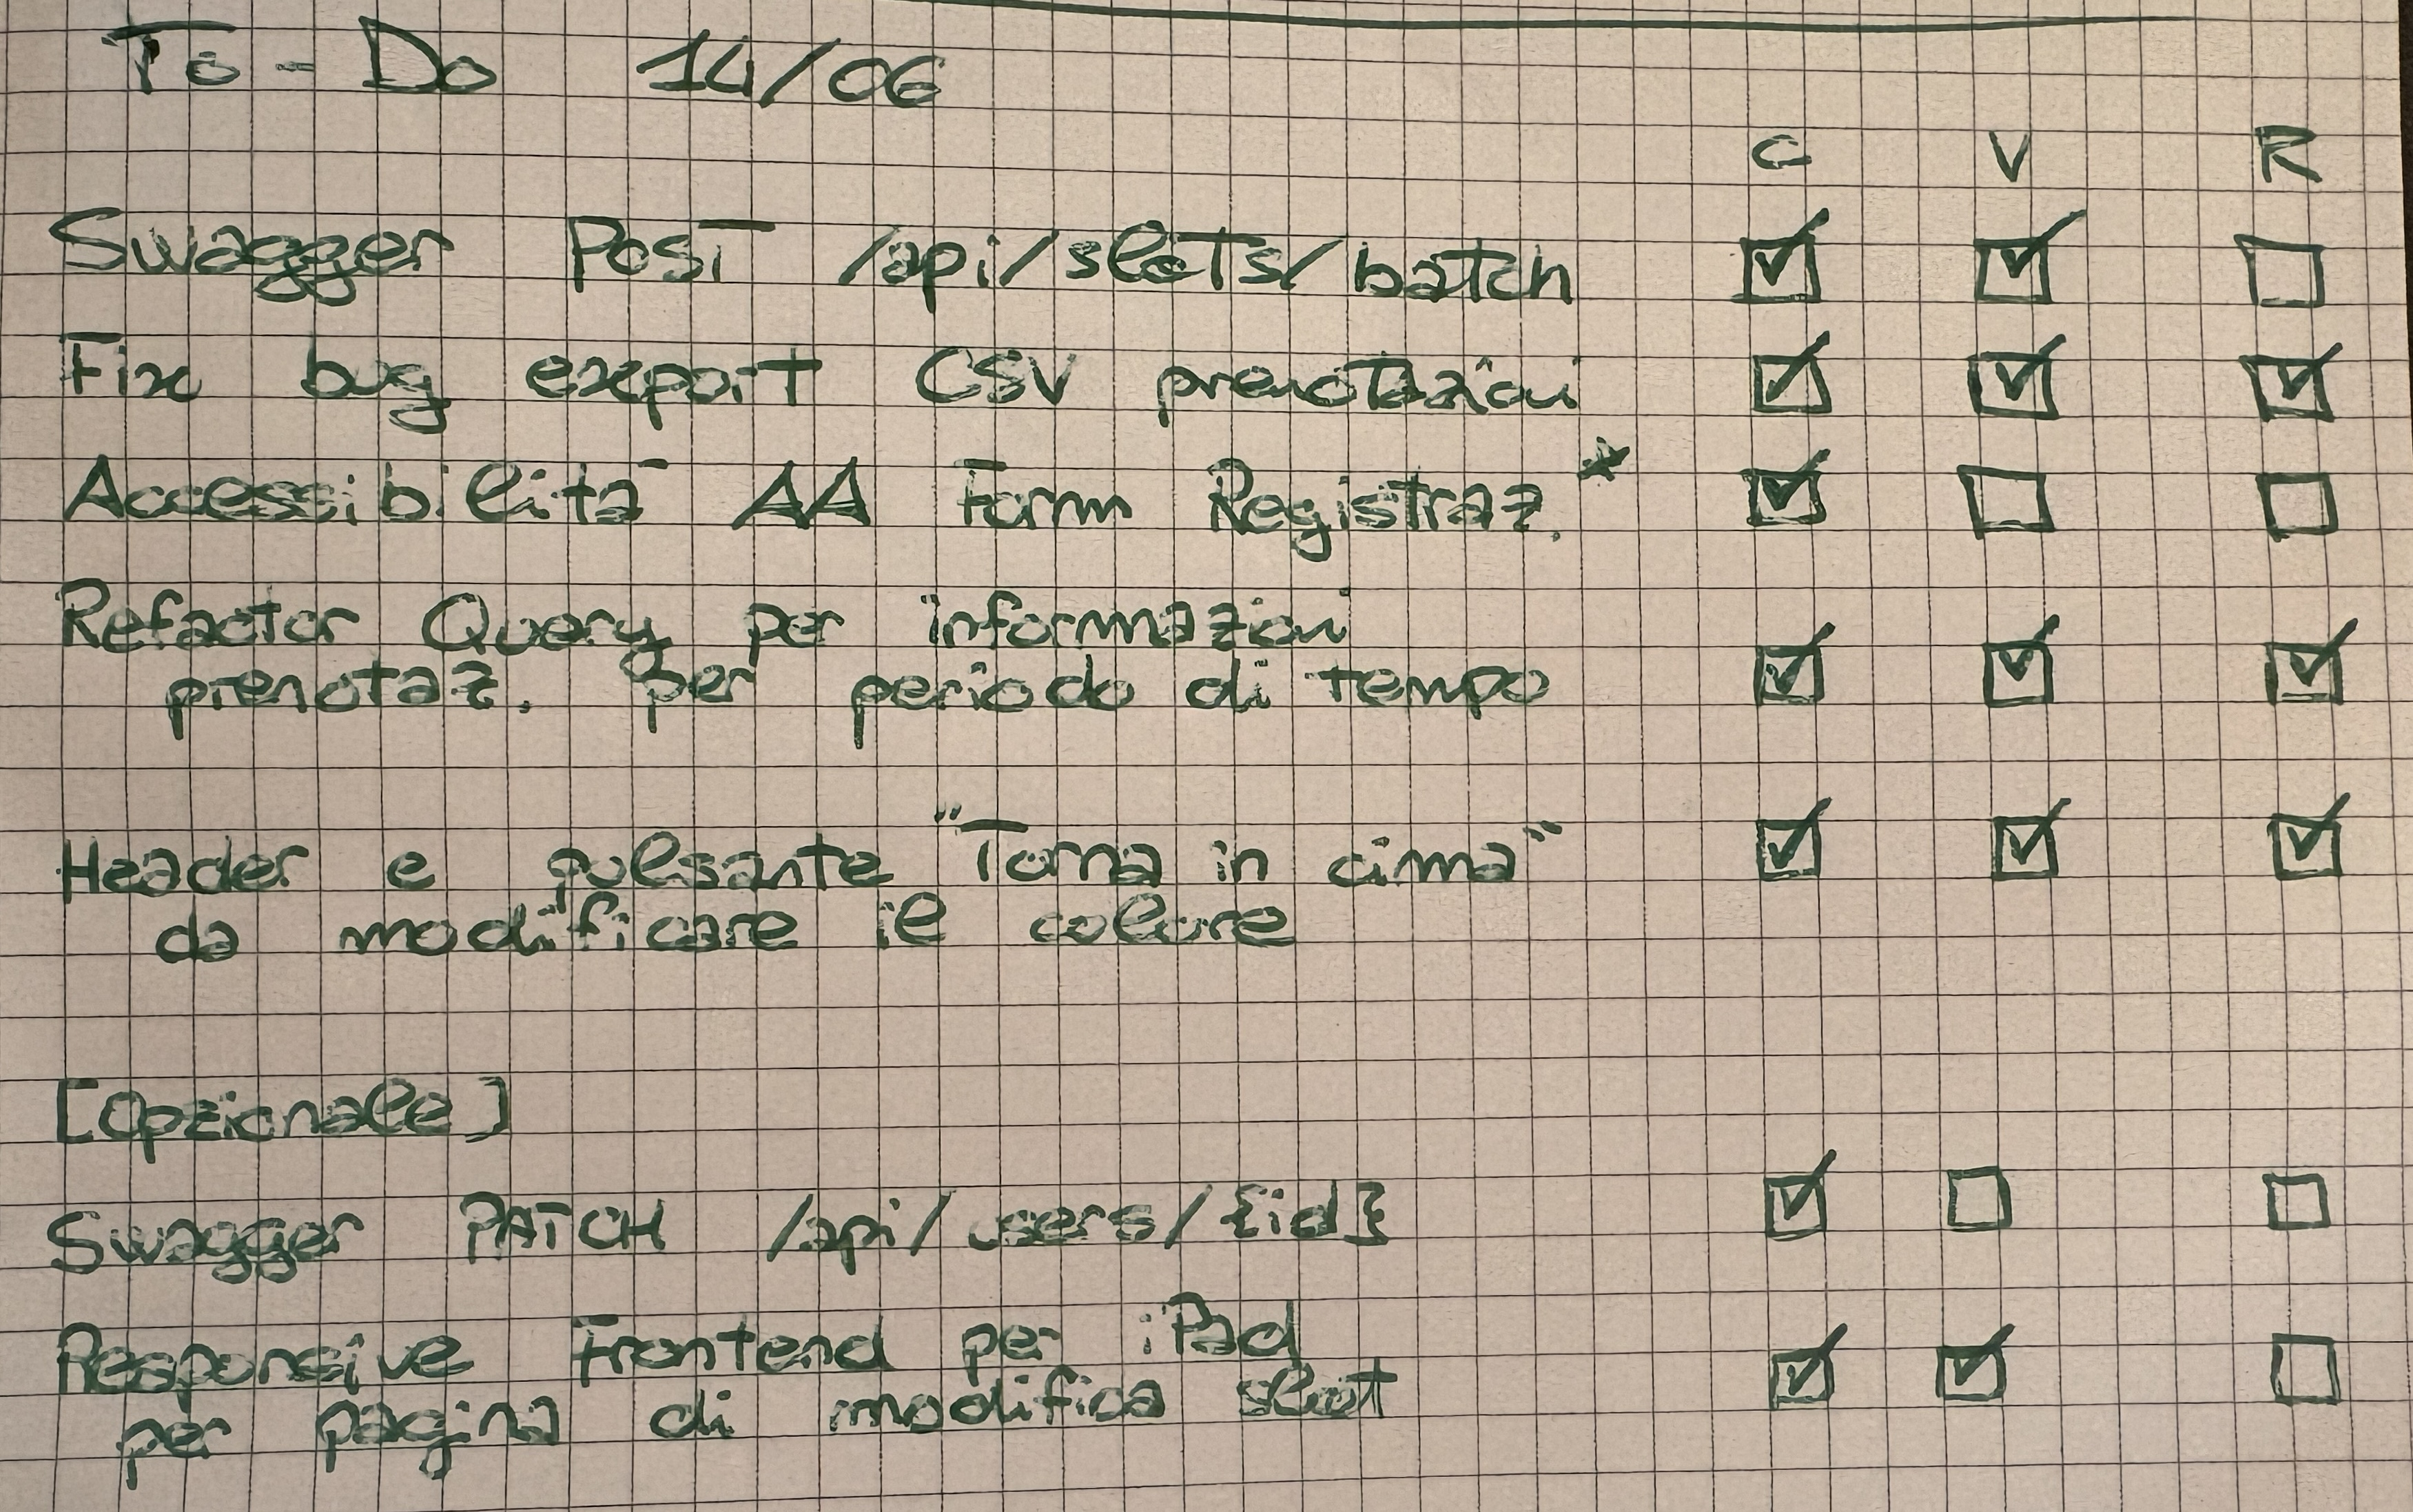
\includegraphics[width=0.7\textwidth]{img/notes.jpg}
    \caption{Appunti cartacei relativi alla fase di analisi del dominio applicativo e modellazione preliminare.}
    \vspace{0.1cm}
    {\footnotesize Elaborazione originale dell'autore\par}
    \label{fig:appunti_analisi}
\end{figure}

\begin{figure}[H]
    \centering
    \includegraphics[width=0.7\textwidth]{img/analysis.png}
    \caption{Sistema di tracciamento giornaliero basato su criteri di completamento, verifica e revisione.}
    \vspace{0.1cm}
    {\footnotesize Elaborazione originale dell'autore\par}
    \label{fig:todo_list}
\end{figure}

La natura esplorativa del progetto ha richiesto inoltre una costante attività di auto-formazione. Ho supportato ogni fase di implementazione mediante la consultazione sistematica delle documentazioni ufficiali delle tecnologie adottate: la guida di riferimento di React \cite{react_docs}, il portale di Microsoft Learn per l'ecosistema .NET \cite{dotnet_docs} e la documentazione tecnica di Informix \cite{informix_docs}. Tale pratica non ha rappresentato un mero supporto all'implementazione, ma un'attività di analisi tecnica strutturata per comprendere le \textit{best practice} di ogni \textit{framework} e applicarle correttamente nel contesto aziendale.

\section{Il ciclo di vita e le sfide progettuali}
\label{sec:ciclo_vita_kargo}

Di seguito dettaglio come ho trasformato le specifiche iniziali in un applicativo funzionante, seguendo la sequenza analisi, progettazione, programmazione e verifica, e motivando le principali decisioni tecniche adottate.

\subsection{Analisi dei requisiti e validazione del prototipo}
\label{subsec:analisi_validazione}

Prima di avviare lo sviluppo vero e proprio, il tutor mi ha formalizzato i vincoli architetturali discussi nel capitolo precedente, introducendomi al progetto con il suo nome provvisorio: "\textit{Web Service} Prenotazione Scarichi". L'obiettivo primario consisteva nel fornire ai corrieri una piattaforma per registrarsi e prenotare le baie dei depositi, centralizzando il controllo delle richieste.

Sfruttando l'assenza di linee guida aziendali rigide per la stesura della documentazione preliminare, ho applicato i principi appresi nel corso di Ingegneria del \textit{Software} per condurre un'analisi dei requisiti strutturata. Ho adottato un approccio gerarchico: sono partito dalla definizione degli attori di sistema, per poi isolare le macro-operazioni e descrivere infine il flusso operativo sequenziale necessario all'utente per completare ogni azione. Questo metodo ha consentito di granulare i requisiti in maniera precisa, rendendoli direttamente implementabili e verificabili attraverso le \textit{checklist} giornaliere descritte nella Sezione~\ref{subsec:sviluppo_personale}.

Ho redatto un documento contenente questa descrizione del dominio, formulando i diagrammi dei casi d'uso tramite PlantUML --- uno strumento che genera diagrammi UML a partire da una sintassi testuale --- per tracciare visivamente ogni scenario di interazione. Successivamente, ho mappato i requisiti, consolidandoli all'interno di apposite tabelle di classificazione. La Figura~\ref{fig:diagramma_casi_uso} e la Figura~\ref{fig:requirements_table} mostrano un estratto del lavoro di analisi.

\begin{figure}[H]
    \centering
    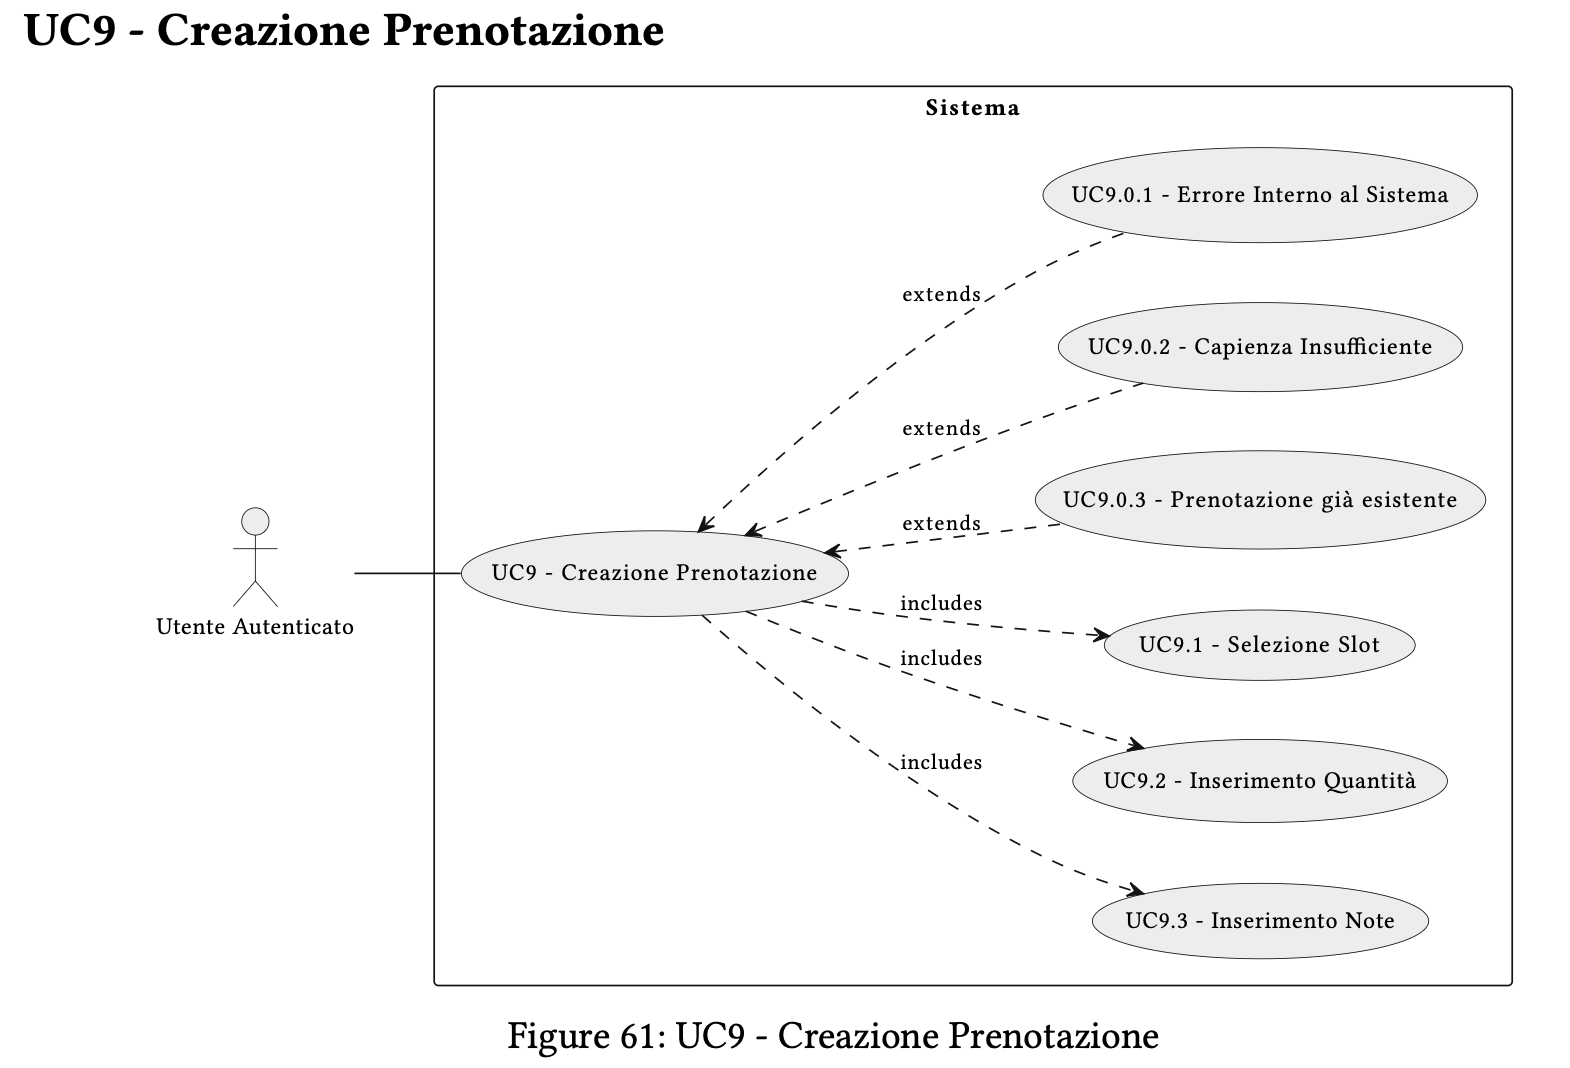
\includegraphics[width=0.7\textwidth]{img/uc.png}
    \caption{Estratto del diagramma dei casi d'uso generato tramite PlantUML.}
    \vspace{0.1cm}
    {\footnotesize Elaborazione originale dell'autore\par}
    \label{fig:diagramma_casi_uso}
\end{figure}

\begin{figure}[H]
    \centering
    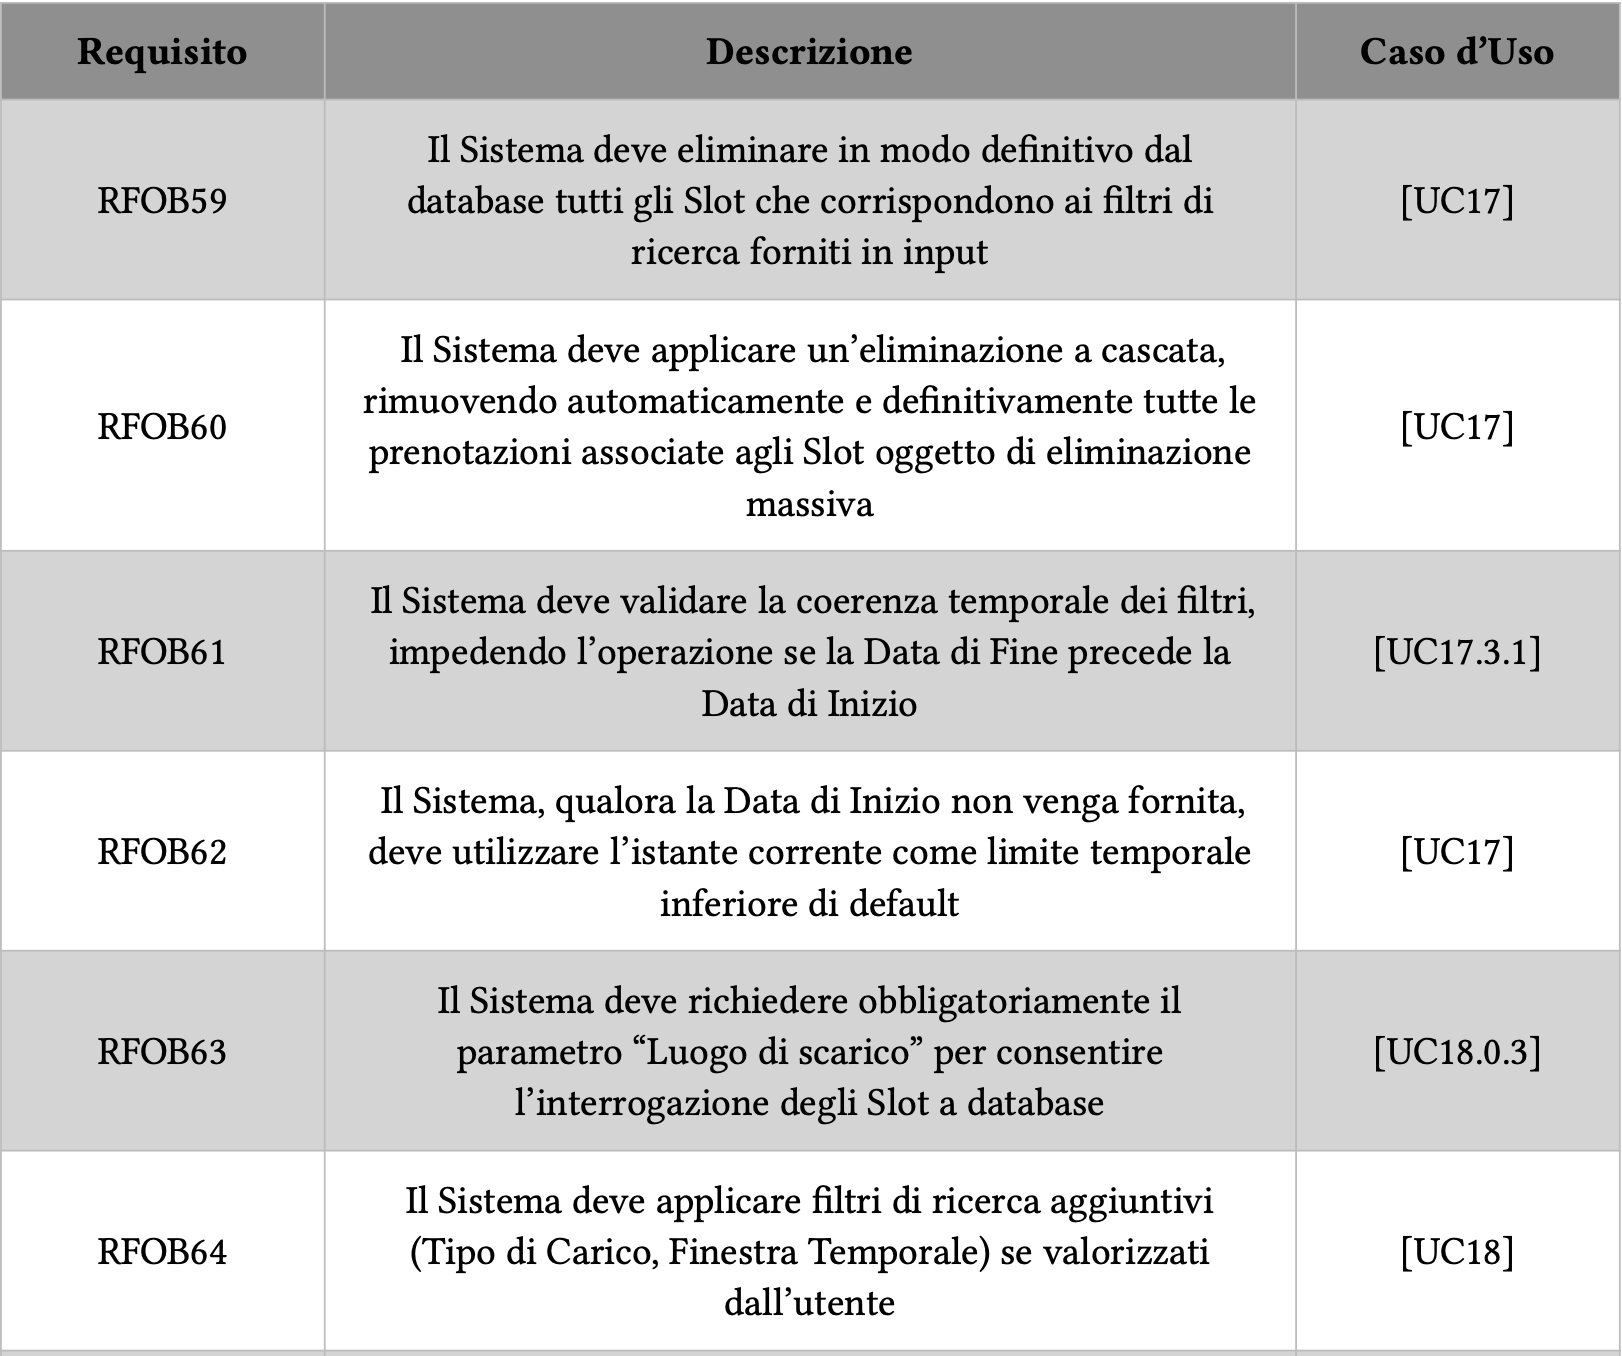
\includegraphics[width=0.8\textwidth]{img/requirements.png}
    \caption{Estratto della tabella di tracciamento dei requisiti funzionali.}
    \vspace{0.1cm}
    {\footnotesize Elaborazione originale dell'autore\par}
    \label{fig:requirements_table}
\end{figure}

Inizialmente, la mia propensione per la documentazione formale e la totale assenza di conoscenze pregresse sui linguaggi C\# e React hanno suscitato alcune perplessità nel tutor aziendale. Tuttavia, esaminando la precisione dei documenti prodotti, egli ha compreso il valore del rigore analitico e mi ha incitato a proseguire con questa metodologia.

Forte dei requisiti validati, ho sviluppato in circa tre settimane un primo prototipo funzionante, con lo scopo di acquisire dimestichezza con lo \textit{stack} tecnologico. Durante la stesura di questo eseguibile preliminare, ho ideato il nome definitivo dell'applicativo --- Kargo --- e ne ho disegnato il logo ufficiale, richiamando la veste cromatica dell'azienda committente, come illustrato in Figura~\ref{fig:logo_kargo}.

\begin{figure}[H]
    \centering
    
\includegraphics[width=0.4\textwidth]{img/KargoLogo.png}
    \caption{Logo dell'applicativo Kargo.}
    \vspace{0.1cm}
    {\footnotesize Elaborazione originale dell'autore\par}
    \label{fig:logo_kargo}
\end{figure}

\subsection{Evoluzione del dominio applicativo e sicurezza}
\label{subsec:evoluzione_dominio}

La rapidità con cui ho consegnato il prototipo ha fornito alla dirigenza tecnica l'opportunità di espandere il raggio d'azione di Kargo. Il tutor ha spostato l'attenzione dal semplice utilizzatore finale alla figura dell'amministratore, con l'intento di rendere il sistema autosufficiente e capace di autogestirsi integralmente.

Ho implementato funzionalità che garantiscono agli amministratori il controllo completo sulle prenotazioni e sugli intervalli temporali, operando sia su singole istanze sia tramite elaborazioni massive (\textit{batch}). Per potenziare il supporto decisionale, ho integrato procedure di esportazione dei dati in formato PDF e CSV, consentendo agli amministratori di estrarre \textit{report} dettagliati delle prenotazioni associate a ogni specifico \textit{slot}. Inoltre, per agevolare l'auto-formazione degli utenti, ho introdotto un modulo di consultazione documentale che espone dinamicamente il manuale utente o il manuale amministratore in base al profilo di autorizzazione del soggetto autenticato.

Parallelamente, ho rilevato la necessità di innalzare gli standard di sicurezza. Ho integrato un sistema di validazione visiva (\textit{captcha}) per scongiurare registrazioni automatizzate da parte di \textit{bot}. Inoltre, il tutor ha imposto un meccanismo di attivazione degli account tramite \gls{otp} --- ovvero un codice numerico monouso --- per prevenire furti d'identità aziendale. 

Per la gestione delle sessioni, ho contestato l'approccio iniziale che prevedeva il passaggio di dati sensibili in chiaro tramite richieste HTTP GET, proponendo e implementando in sua sostituzione l'adozione di \gls{jwt} --- token crittografici compatti impiegati per il trasferimento sicuro di asserzioni tra le parti --- strutturati in \textit{Access} e \textit{Refresh Token} e archiviati in \textit{cookie} \textit{HttpOnly}, inaccessibili agli \textit{script} lato \textit{client}.

\subsection{Progettazione architetturale e direttive di codifica}
\label{subsec:architettura_codifica}

L'evoluzione dei requisiti ha progressivamente concentrato la complessità del sistema nelle regole di dominio, rendendo inefficace un approccio procedurale classico. Ho pertanto adottato il modello di sviluppo guidato dal dominio (\gls{ddd}), necessario per governare vincoli stringenti: le prenotazioni dovevano rispettare un tempo limite di registrazione; il sistema doveva condizionare dinamicamente le operazioni permesse in base allo stato dell'utente; la generazione \textit{batch} richiedeva controlli incrociati per impedire sovrapposizioni e rispettare il limite massimo di porte disponibili.

Per proteggere questa logica di \textit{business}, ho adottato l'architettura esagonale (\textit{Ports and Adapters}): l'utilizzo di interfacce, ovvero le porte, ha delegato a specifici \textit{adapter} la responsabilità di dialogare con la base dati corretta, rendendo il sistema agnostico rispetto alle differenze strutturali tra il \textit{database} di collaudo e quello di produzione. Tramite PlantUML ho strutturato i diagrammi delle classi partendo dal \textit{Domain Layer}, fino ai \textit{Controller} (Figura~\ref{fig:diagramma_classi}).

\begin{figure}[H]
    \centering
    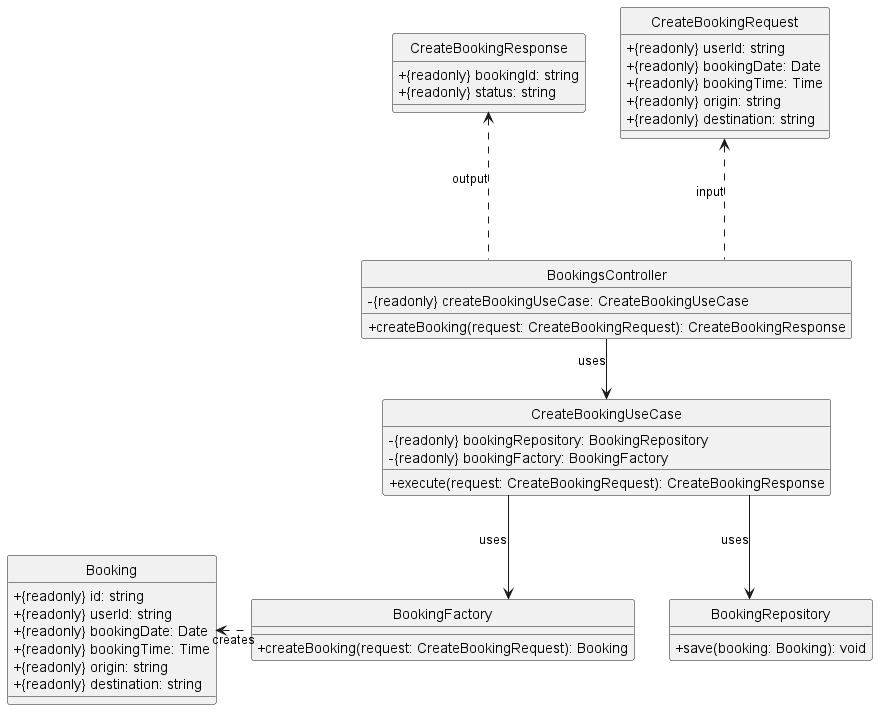
\includegraphics[width=0.8\textwidth]{img/design.jpeg}
    \caption{Modellazione delle classi di dominio e del livello applicativo.}
    \vspace{0.1cm}
    {\footnotesize Elaborazione originale dell'autore\par}
    \label{fig:diagramma_classi}
\end{figure}

Nella stesura del codice, ho applicato i principi \gls{solid} per la creazione di \textit{software} manutenibile e disaccoppiato:
\begin{itemize}
    \item \textbf{Inversione del controllo e iniezione delle dipendenze:} ho svincolato le classi dalla loro implementazione concreta mediante interfacce astratte, garantendo modularità e intercambiabilità.
    \item \textbf{Responsabilità singola:} ogni entità assolve esclusivamente a un singolo compito logico.
    \item \textbf{Segregazione e Sostituzione di Liskov:} il codice di dominio interagisce con interfacce minimali, delegando agli \textit{adapter} la traduzione dei contratti astratti.
\end{itemize}

Sul livello \textit{frontend} in React e TypeScript, ho configurato un ambiente di analisi statica (\textit{linting}) tramite ESLint e Prettier. Infine, per preservare le prestazioni, ho implementato un gestore universale delle eccezioni --- evitando la duplicazione di costrutti \texttt{try-catch} in violazione del principio \gls{dry} --- e un \textit{rate limiter} sulle \gls{api} per proteggere le operazioni critiche.

A titolo esemplificativo, la Figura~\ref{fig:create_booking_usecase} riporta l'implementazione del caso d'uso primario per la generazione delle prenotazioni. Il frammento evidenzia l'applicazione pratica dell'Iniezione delle Dipendenze --- le interfacce di accesso ai dati vengono passate al costruttore --- e l'incapsulamento delle regole di \textit{business}. Il sistema delega la persistenza agli \textit{adapter} infrastrutturali tramite il \textit{pattern Unit of Work} esclusivamente dopo aver validato rigorosamente i vincoli di dominio (quali lo stato dell'utente, la capienza dello \textit{slot} e le tempistiche di scarico).

\begin{figure}[H]
    \centering
    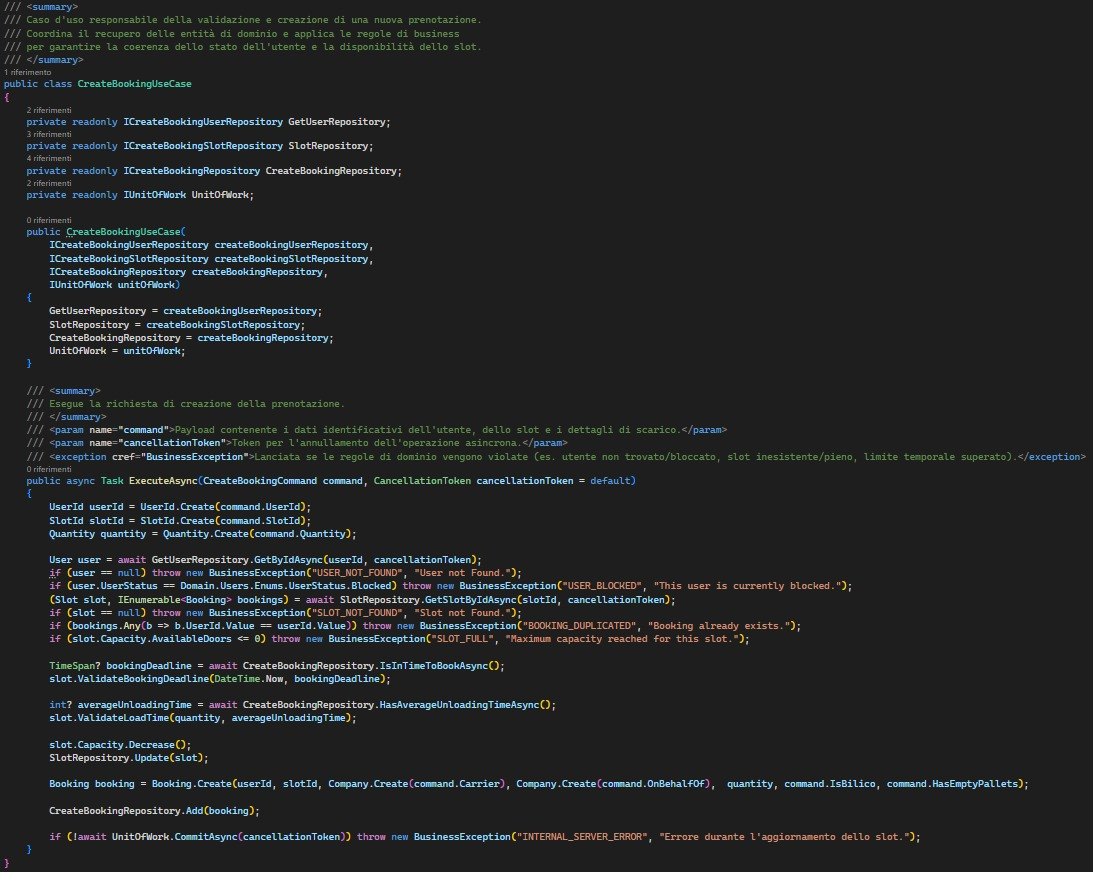
\includegraphics[width=1.0\textwidth]{img/code.jpeg}
    \caption{Implementazione del caso d'uso di creazione prenotazione.}
    \vspace{0.1cm}
    {\footnotesize Elaborazione originale dell'autore\par}
    \label{fig:create_booking_usecase}
\end{figure}

\subsection{Verifica e validazione delle funzionalità}
\label{subsec:verifica_validazione}

Ho interpretato la fase di verifica come un elemento strutturale continuo del ciclo di sviluppo. Ho condotto la validazione dei requisiti in modo strettamente incrementale, sottoponendo ogni funzionalità implementata a riscontri operativi diretti per garantirne la piena conformità.

Per collaudare il \textit{backend}, mi sono avvalso principalmente di Postman per simulare i percorsi tracciati nei diagrammi dei casi d'uso e di Swagger per documentare e testare attivamente gli \textit{endpoint} esposti. Sul versante \textit{frontend}, ho validato l'applicativo tramite esecuzioni dirette nell'ambiente di sviluppo locale, focalizzandomi sull'accessibilità visiva e comportamentale con il supporto dei DevTools di Google Chrome. Ho verificato la reattività (\textit{responsiveness}) dell'applicativo su schermi \textit{desktop}, \textit{tablet} e terminali mobili. 

Sebbene abbia strutturato l'ambiente TypeScript per supportare la scrittura di \textit{unit test} al fine di garantire una solida base per future integrazioni, la validazione del presente prototipo si è basata su un collaudo empirico iterativo, integrato dalle revisioni periodiche condivise con il tutor aziendale per stabilire l'approvazione funzionale dei moduli.

\section{Risultati qualitativi e quantitativi}
\label{sec:risultati_kargo}

Al termine delle ore previste per la stesura del codice, ho sottoposto l'applicativo Kargo alla valutazione finale della dirigenza tecnica. L'esito del progetto si articola su due dimensioni d'analisi: la percezione del prodotto dal lato utente e la misurazione delle metriche ingegneristiche di copertura.

\subsection{Il prodotto dal lato utente}
\label{subsec:risultati_qualitativi}

Sul piano qualitativo, Kargo si presenta come un applicativo reattivo, solido e fortemente orientato all'usabilità. Sebbene abbia sviluppato l'applicativo per l'uso interno logistico --- un settore che spesso subordina l'estetica alla pura funzionalità --- ho dedicato particolare attenzione all'interfaccia utente, garantendo il rispetto degli standard di accessibilità \textit{Web Content Accessibility Guidelines} (WCAG) di livello AA e, in alcuni componenti critici, di livello AAA. Ho verificato tale conformità analizzando i rapporti di contrasto cromatico, implementando la navigazione completa tramite tastiera e utilizzando i \textit{tag} semantici HTML5 controllati mediante gli strumenti di ispezione del \textit{browser}.

L'interfaccia guida gli attori del sistema attraverso flussi operativi chiari. Per gestire la notevole mole di dati derivante dall'espansione del dominio, ho progettato e implementato funzioni avanzate di ricerca e filtraggio dinamico. Sia i corrieri, nella consultazione degli \textit{slot} liberi, sia gli amministratori, nel monitoraggio globale del deposito, possono interrogare la base dati in tempo reale, isolando le prenotazioni per data, stato o tipologia di carico con risposte visive immediate. 

Le Figure dalla~\ref{fig:kargo_selezione_slot} alla~\ref{fig:kargo_modifica_slot} dimostrano la resa finale dell'applicativo, evidenziando la funzionalità di creazione della prenotazione lato corriere e di gestione delle prenotazioni lato amministratore.

\begin{figure}[H]
    \centering
    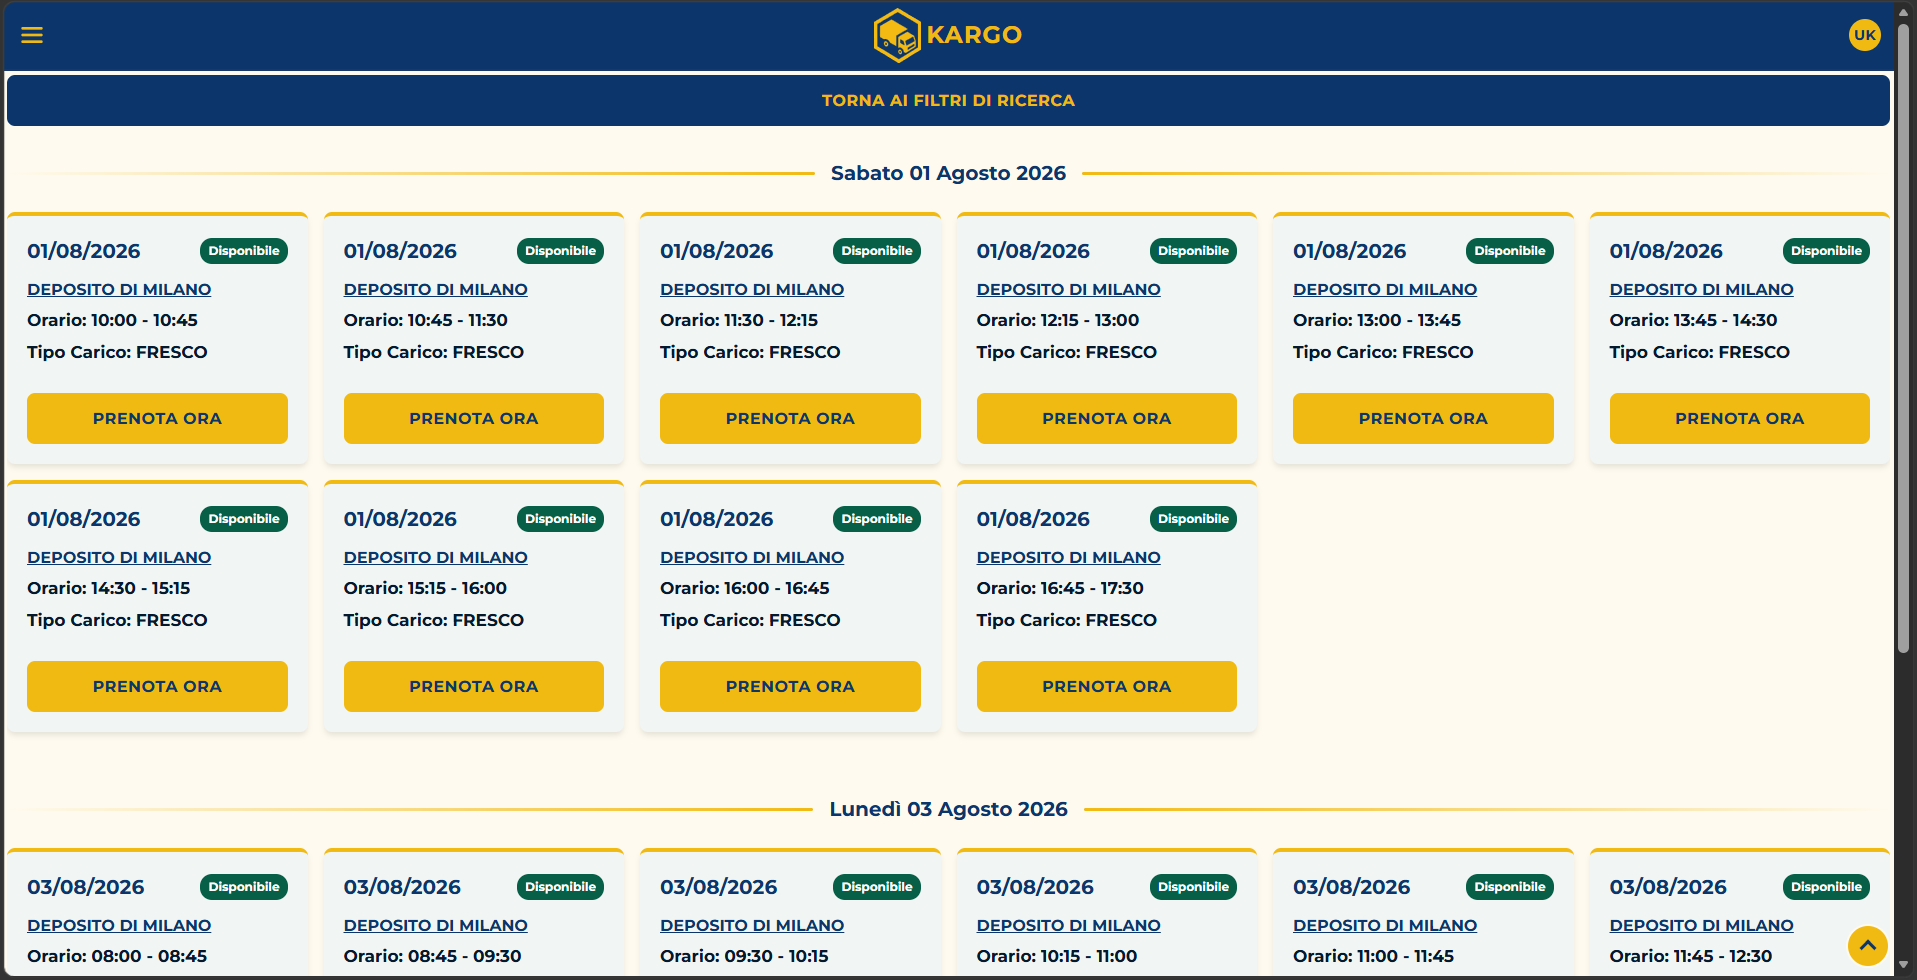
\includegraphics[width=1.0\textwidth]{img/viewSlotsForBookingPage2.png} 
    \caption{Interfaccia di selezione della finestra temporale di prenotazione.}
    \vspace{0.1cm}
    {\footnotesize Elaborazione originale dell'autore\par}
    \label{fig:kargo_selezione_slot}
\end{figure}

\begin{figure}[H]
    \centering
    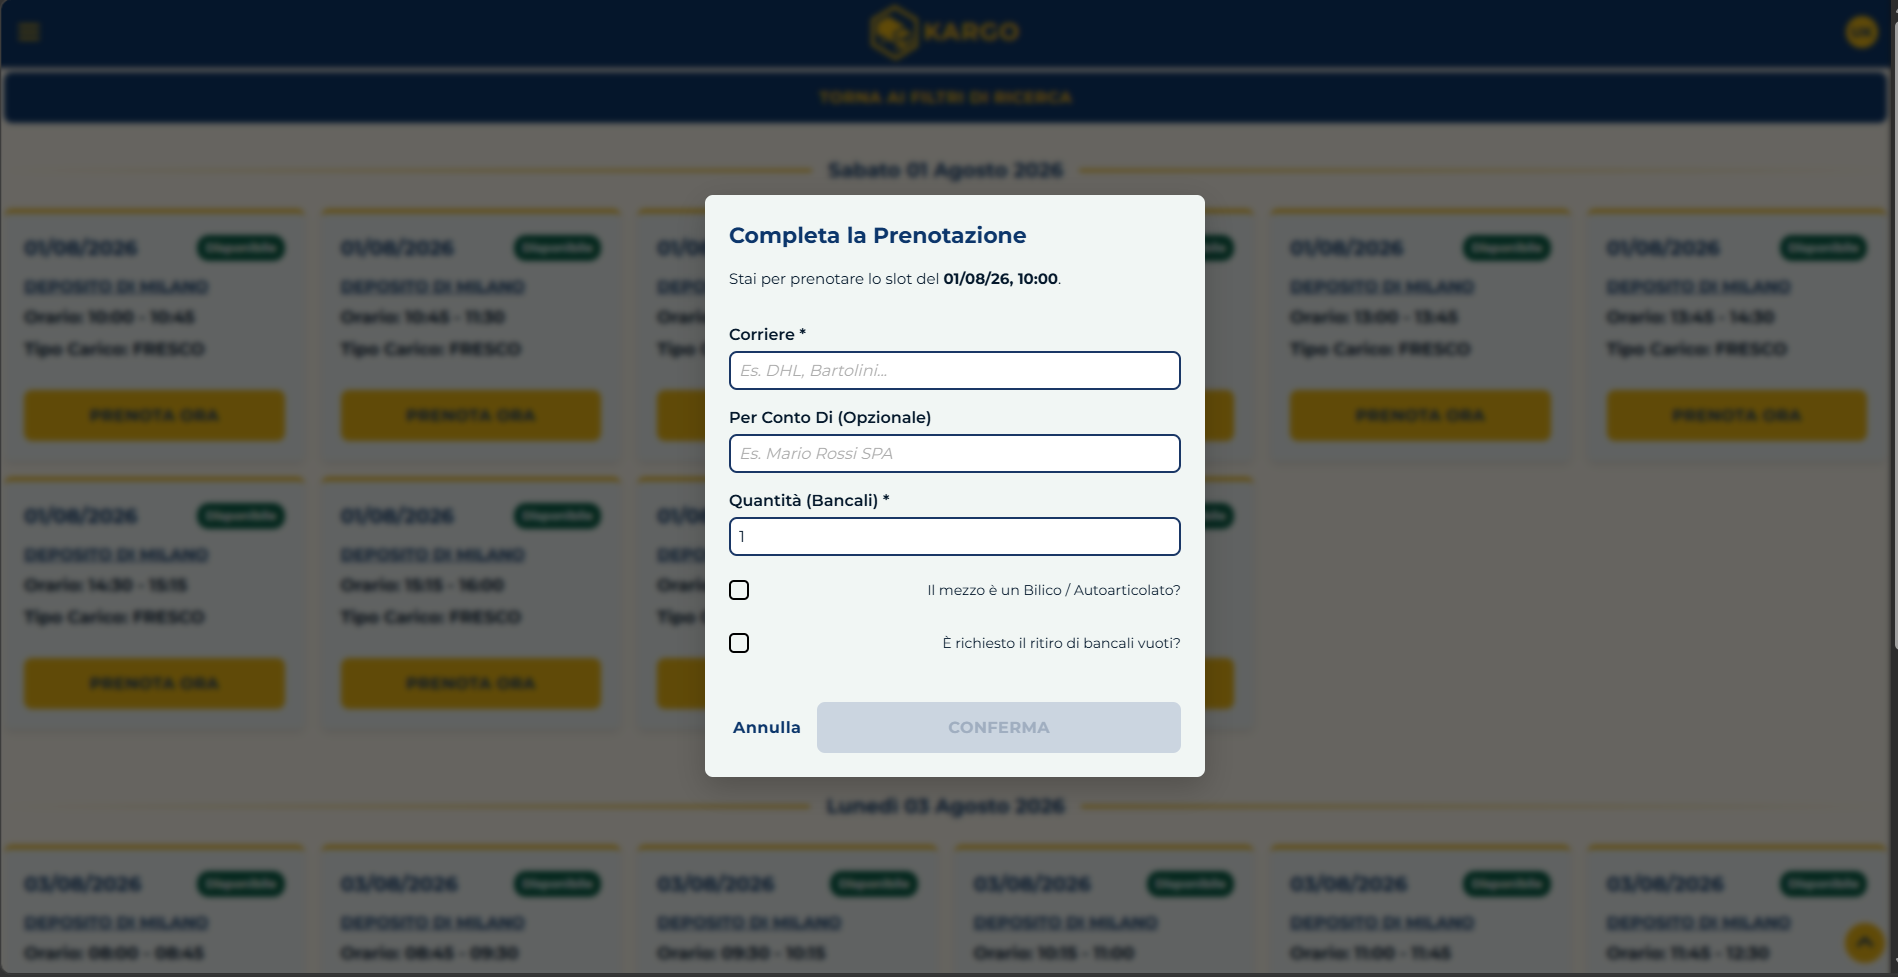
\includegraphics[width=0.9\textwidth]{img/completeBooking.png} 
    \caption{Dettaglio sul completamento della prenotazione.}
    \vspace{0.1cm}
    {\footnotesize Elaborazione originale dell'autore\par}
    \label{fig:kargo_completamento_prenotazione}
\end{figure}

\begin{figure}[H]
    \centering
    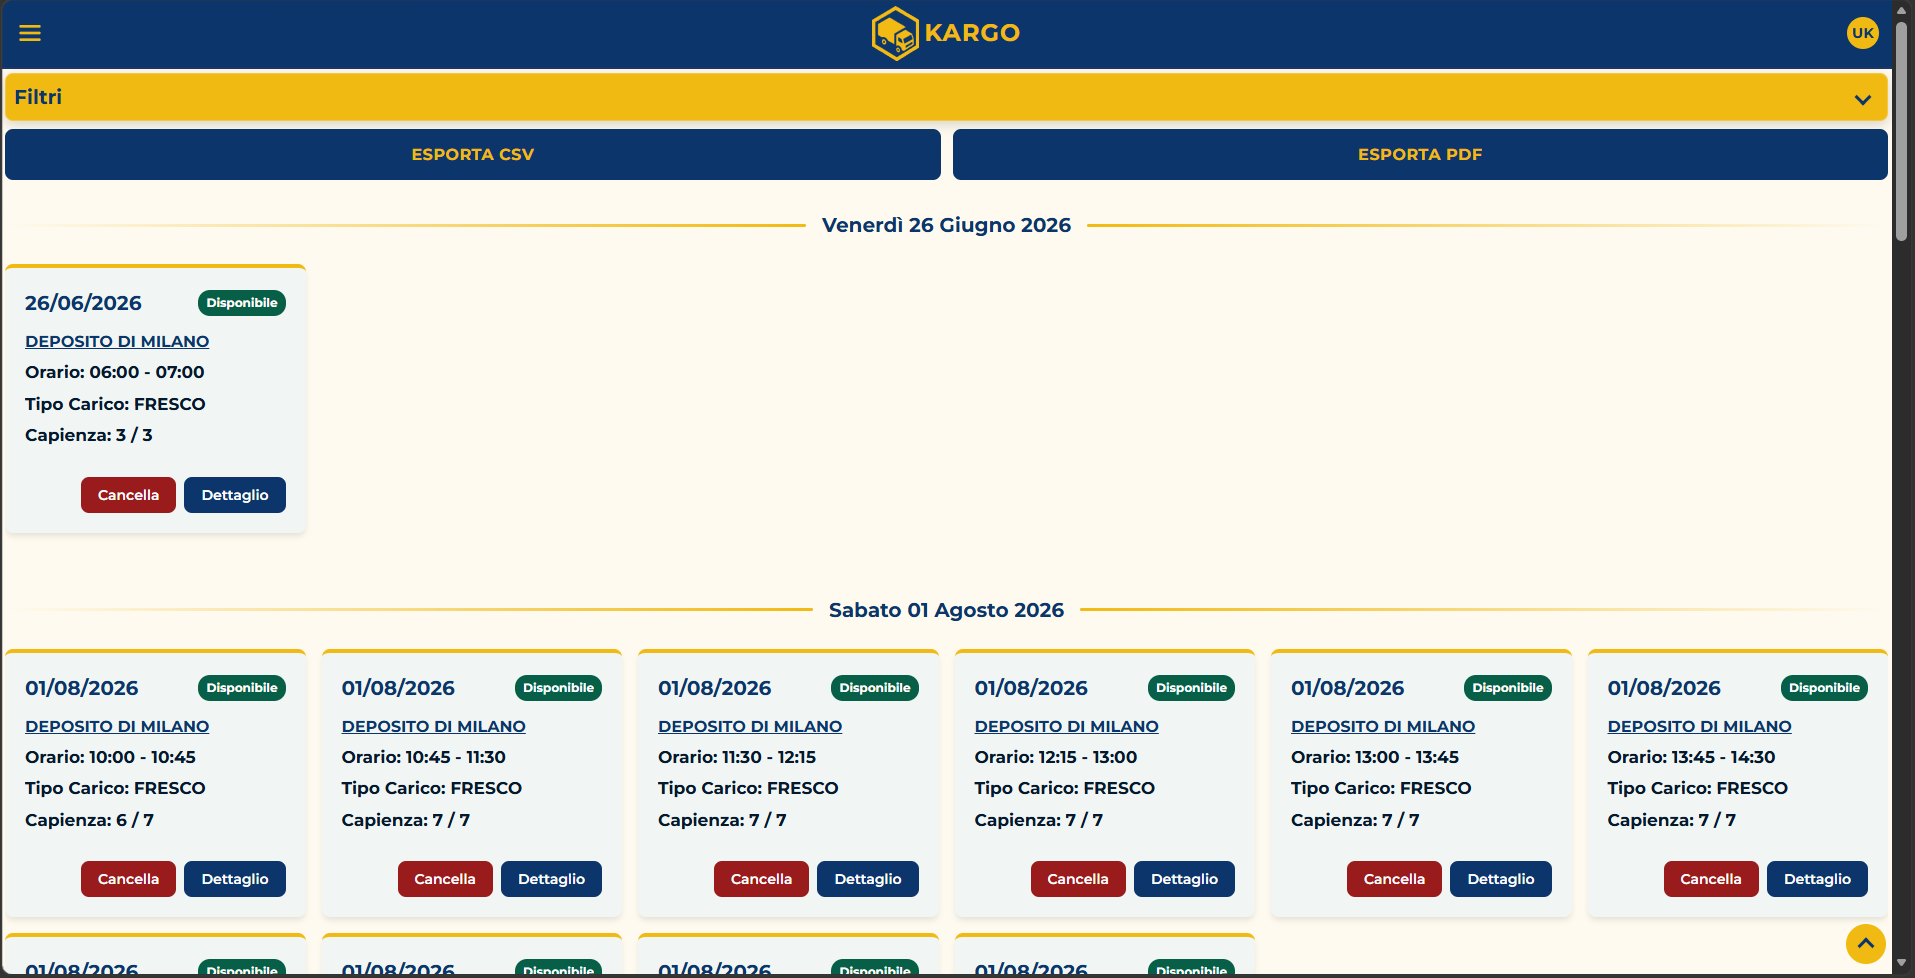
\includegraphics[width=0.9\textwidth]{img/viewSlotsPage2.png} 
    \caption{Visualizzazione della gestione degli slot temporali.}
    \vspace{0.1cm}
    {\footnotesize Elaborazione originale dell'autore\par}
    \label{fig:kargo_gestione_slot}
\end{figure}

\begin{figure}[H]
    \centering
    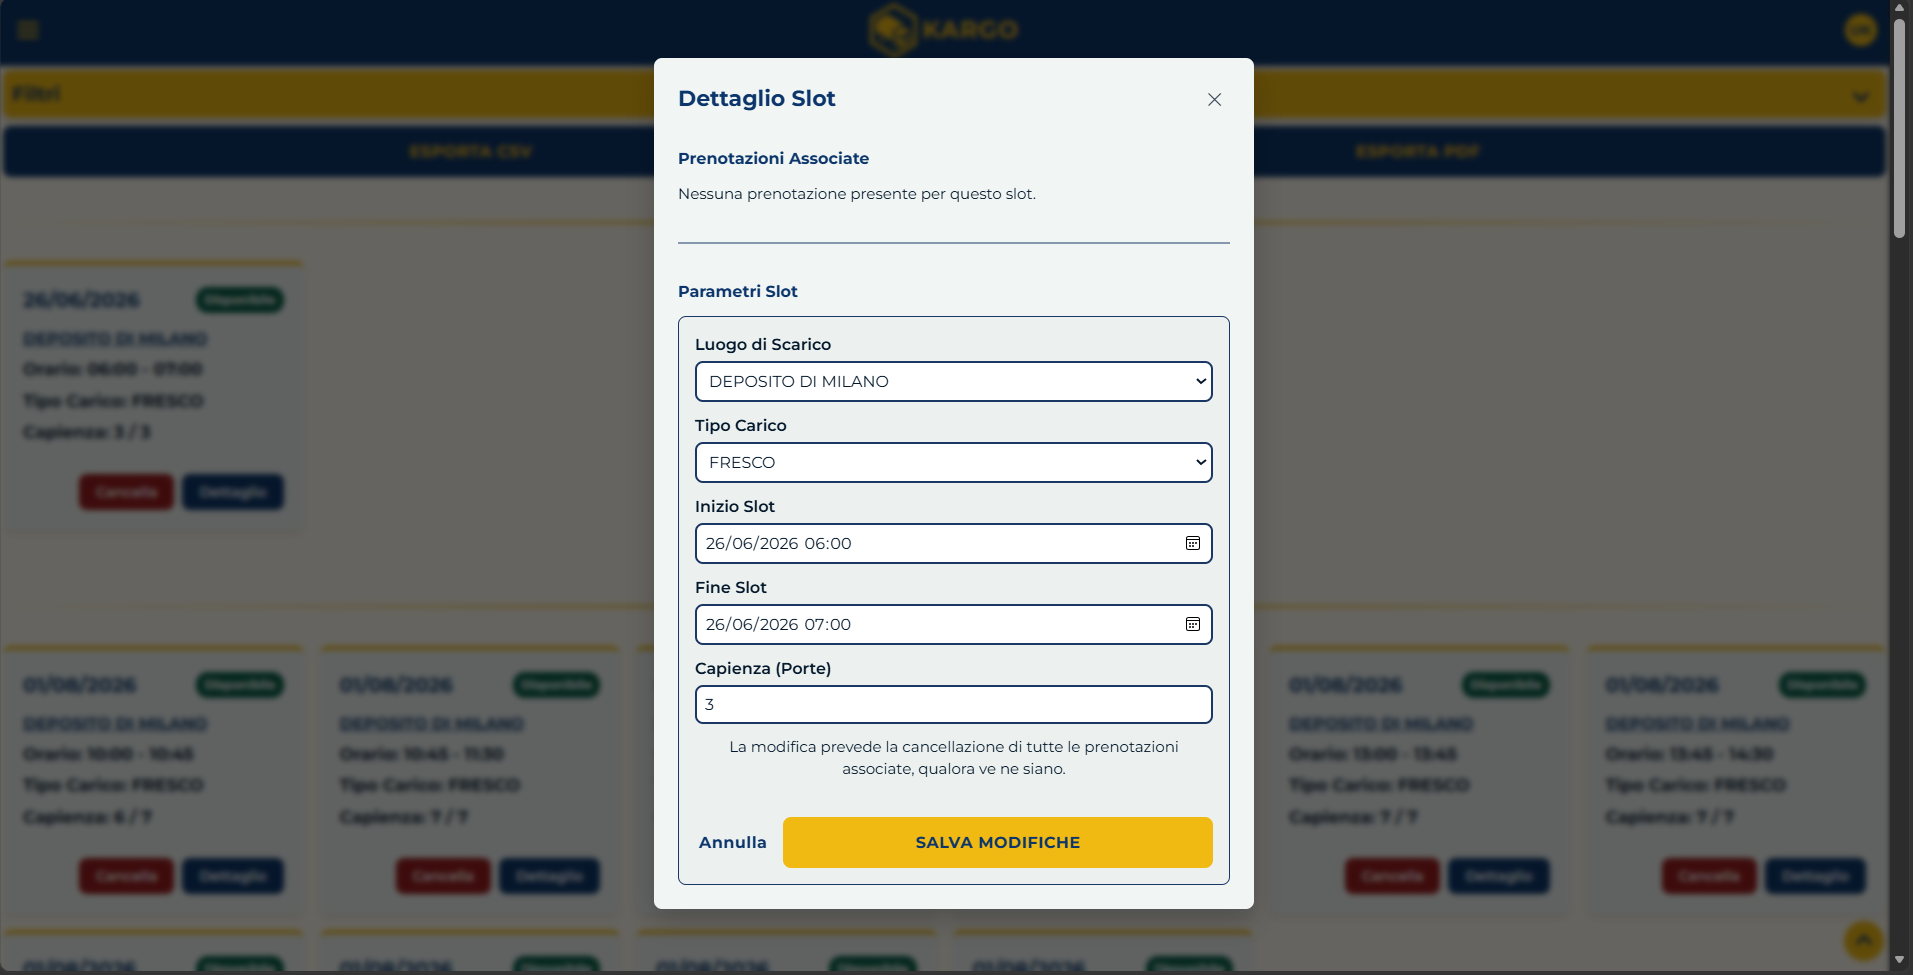
\includegraphics[width=0.9\textwidth]{img/modifySlot.png} 
    \caption{Dettaglio sulla gestione degli slot temporali.}
    \vspace{0.1cm}
    {\footnotesize Elaborazione originale dell'autore\par}
    \label{fig:kargo_modifica_slot}
\end{figure}

\subsection{Copertura e metriche di progetto}
\label{subsec:risultati_quantitativi}

Sotto il profilo quantitativo, i risultati testimoniano il pieno conseguimento degli obiettivi aziendali e l'efficacia strategica dello \textit{stage} delineati nel Capitolo~\ref{chap:strategia}. Nonostante il tutor abbia richiesto un massiccio ampliamento del dominio a lavori già avviati, ho consegnato la \textit{release} definitiva dell'applicativo con circa una settimana di anticipo rispetto alle scadenze originarie concordate con l'azienda.

Dal punto di vista della copertura funzionale, ho mappato e soddisfatto integralmente le richieste del committente. La Tabella~\ref{tab:riepilogo_requisiti} illustra il riepilogo quantitativo dei requisiti individuati in fase di analisi, suddivisi per tipologia e grado di adempimento.

\begin{table}[H]
    \centering
    \begin{tabular}{p{0.3\textwidth} c c c}
        \hline
        \textbf{Tipologia Requisito} & \textbf{Obbligatori} & \textbf{Desiderabili} & \textbf{Opzionali} \\
        \hline
        Requisiti Utente & 24 & 1 & 1 \\
        Requisiti Funzionali & 80 & 1 & 0 \\
        Requisiti non Funzionali & 3 & 1 & 2 \\
        Requisiti di Interfaccia & 35 & 3 & 1 \\
        \hline
        \textbf{Totale} & \textbf{142} & \textbf{6} & \textbf{4} \\
        \hline
    \end{tabular}
    \caption{Riepilogo quantitativo della tracciabilità dei requisiti di progetto.}
    \vspace{0.1cm}
    {\footnotesize Valori assoluti derivati dalla matrice di tracciamento dei requisiti validata dal tutor aziendale.\par}
    \label{tab:riepilogo_requisiti}
\end{table}

A livello di volumetria del prodotto, il \textit{repository} finale si compone di una ricca infrastruttura logica, quantificabile in circa 20 \textit{endpoint} \gls{api} esposti lato \textit{backend}, supportati da svariate decine di classi di dominio in C\# e molteplici componenti \textit{custom} in React sviluppati \textit{ex novo}. A questa produzione informatica ho affiancato il parallelo lavoro di stesura documentale, concretizzatosi nella redazione formale del documento di analisi dei requisiti iniziale e nella produzione di due guide operative complete: il manuale utente, destinato ai corrieri, e il manuale amministratore, riservato al personale della logistica interna.

Infine, coerentemente con le direttive operative interne descritte nella Sezione~\ref{subsec:verifica_validazione}, non ho prodotto metriche automatizzate di \textit{code-coverage}. Sebbene abbia configurato l'ambiente per supportare rigide analisi statiche mediante ESLint, ho basato la validazione finale sull'esito positivo dei rigorosi collaudi empirici e visivi condotti congiuntamente al \textit{team} tecnico di Ergon Informatica, decretando il successo complessivo dello \textit{stage}.